\begin{activite}[Découvrir les outils de GeoGebra]

	\subsection{les principaux outils}
Commencer par lancer le logiciel GeoGebra. Faire afficher une page blanche à l'aide du menu "affichage", en déselectionnant les axes et/ou grille si besoin.

En parcourant les différents outils de construction disponibles dans la barre d'outils, reliez proprement chaque outil avec l'icône qui lui correspond.

\begin{center}
 \begin{tabularx}{\linewidth}{|r|lXrc}
  \cline{1-1}
  Nouveau point & \huge{\textbullet} & & \huge{\textbullet} & 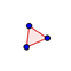
\includegraphics[width=1cm]{geopolygone} \\  \cline{1-1}
  Déplacer la feuille de travail & \huge{\textbullet} & & \huge{\textbullet} & 
\includegraphics[width=1cm]{geoangle} \\ \cline{1-1}
  Demi-droite passsant par deux points & \huge{\textbullet} & & \huge{\textbullet} & 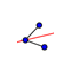
\includegraphics[width=1cm]{geobissectrice} \\ \cline{1-1}
  Droite perpendiculaire & \huge{\textbullet} & & \huge{\textbullet} & 
\includegraphics[width=1cm]{geosegment} \\ \cline{1-1}
  Angle & \huge{\textbullet} & & \huge{\textbullet} & 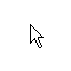
\includegraphics[width=1cm]{geofleche} \\ \cline{1-1}
  Milieu ou centre & \huge{\textbullet} & & \huge{\textbullet} & 
\includegraphics[width=1cm]{geopoint} \\ \cline{1-1}
  Droite passant par deux points & \huge{\textbullet} & & \huge{\textbullet} & 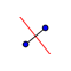
\includegraphics[width=1cm]{geomediatrice} \\ \cline{1-1}
  Segment entre deux points & \huge{\textbullet} & & \huge{\textbullet} & 
\includegraphics[width=1cm]{geodemidroite} \\ \cline{1-1}
  Déplacer & \huge{\textbullet} & & \huge{\textbullet} & 
\includegraphics[width=1cm]{geodroite} \\ \cline{1-1}
  Bissectrice & \huge{\textbullet} & & \huge{\textbullet} & 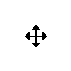
\includegraphics[width=1cm]{geodeplacement} \\ \cline{1-1}
  Médiatrice & \huge{\textbullet} & & \huge{\textbullet} & 
\includegraphics[width=1cm]{geoperpendiculaire} \\ \cline{1-1}
  Polygone & \huge{\textbullet} & & \huge{\textbullet} & 
\includegraphics[width=1cm]{geomilieu} \\ \cline{1-1}
  \end{tabularx}
\end{center}

	\subsection{Construire sa première figure}
En utilisant les commandes de l'exercice précédent, réalise la figure correspondant au programme de construction suivant:
\begin{enumerate}
\item Créer deux points A et B et tracer la droite (AB).
\item Déplacer le point A. La droite (AB) doit se déplacer en suivant le point.
\item Placer un point C tel que $C \notin(AB)$. Tracer la demi-droite [AC) et le segment [BC].
\item Afficher la longeur BC.
\item Placer le milieu I du segment [BC] et afficher le longueur BI.
\item Tracer le cercle de centre A passant par B.
\item Tracer le cercle de centre C, de rayon 4.
\item Fais vérifier ton travail par le professeur.
\end{enumerate}

	\subsection{Reproduire une figure}
\begin{enumerate}
\item Réaliser la figure ci-contre (B est à l'intersection des deux cercles)
\item Déplacer le point B. S'il reste sur les deux cercles alors la figures est juste.
\item Fais vérifier ton travail par le professeur.
\end{enumerate}
\begin{center}
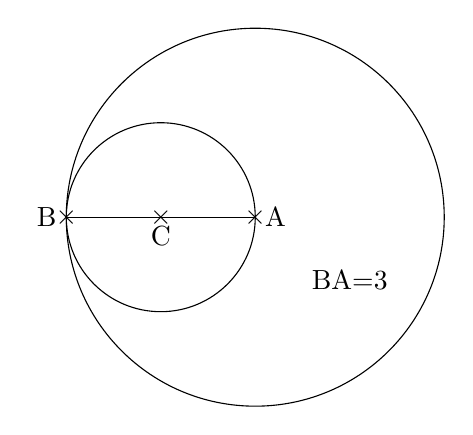
\begin{tikzpicture}[scale=0.8]

\draw (0,0) circle (3);
\draw (-1.5,0) circle (1.5);
\node at (0,0) {$\times$};
\node[right] at (0,0) {A};
\node at (-1.5,0) {$\times$};
\node[below] at (-1.5,0) {C};
\node at (-3,0) {$\times$};
\node[left] at (-3,0) {B};
\draw (-3,0) -- (0,0);
\node at (1.5,-1) {BA=3};
\end{tikzpicture}

\end{center}
\end{activite}

%%%%%%%%%%%%%%%%%%%%%%%%%%%%%%%%%%%%%%%%%%%%%%%%%%%%%%%%%%%%%%%%%%%%%%%%%%%%%%%%%%%%%%%%%%%%%%%%%%


\begin{activite}[À la découverte d'un nouveau code]

  \begin{enumerate}
   \item Lire la consigne de la case \circled{1} et observer la figure correspondant à cette consigne.
Faire de même pour la case \circled{2}.

Quand le code est compris, tracer la figure de la case \circled{3} et écrire la consigne de la case \circled{4}.


  \vspace{1em}
  
  
  
  \begin{tabular}{|c|c|c|c|c|}
  \cline{1-2}\cline{4-5}
    \circled{1} 		& \circled{2} 		& 	& \circled{3} 		& \circled{4}	\\ 
     Tracer $(AB)$ 	&  Tracer $[AC)$ 	& 	& Tracer $(AB)$	& 	 		\\ 
     Tracer $[AC]$ 	& Tracer $[BC]$ 	& 	& Tracer$[BC]$		& 			\\
     				&				&	& Tracer$[AC)$		&			\\ \cline{1-2}\cline{4-5}
   %manuel 6e, chapitre G3
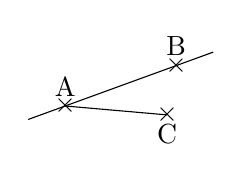
\begin{tikzpicture}[scale=1,every node/.style={scale=1}]

\draw (0,0) node [above]{A};
\draw (0,0) node {$\times$};
\draw (20:1.5) node [above]{B};
\draw (20:1.5) node {$\times$};
\draw (-5:1.3) node [below]{C};
\draw (-5:1.3) node {$\times$};

\draw (0,0)--+(200:0.5)--(20:1.5)--+(20:0.5);
\draw (0,0)--(-5:1.3);

\draw (0,0.7); %pour donner un peu plus de hauteur à l'image
\end{tikzpicture} 
 & 
   %manuel 6e, chapitre G3
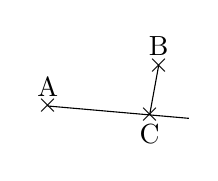
\begin{tikzpicture}[scale=1,every node/.style={scale=1}]

\draw (0,0) node [above]{A};
\draw (0,0) node {$\times$};
\draw (20:1.5) node [above]{B};
\draw (20:1.5) node {$\times$};
\draw (-5:1.3) node [below]{C};
\draw (-5:1.3) node {$\times$};

\draw (20:1.5)--(-5:1.3);
\draw (0,0)--(-5:1.8);

\draw (0,0.7); %pour donner un peu plus de hauteur à l'image
\end{tikzpicture} 
 & & 
   %manuel 6e, chapitre G3
\begin{tikzpicture}[scale=1,every node/.style={scale=1}]

\draw (0,0) node [above]{A};
\draw (0,0) node {$\times$};
\draw (20:1.5) node [above]{B};
\draw (20:1.5) node {$\times$};
\draw (-5:1.3) node [below]{C};
\draw (-5:1.3) node {$\times$};

%\draw (20:1.5)--(-5:1.3);
%\draw (0,0)--(-5:1.8);

\draw (0,1.5); %pour donner un peu plus de hauteur à l'image
\end{tikzpicture} 
& 
   %manuel 6e, chapitre G3
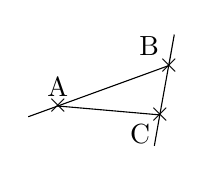
\begin{tikzpicture}[scale=1,every node/.style={scale=1}]

\draw (0,0) node [above]{A};
\draw (0,0) node {$\times$};
\draw (20:1.5) node [above left]{B};
\draw (20:1.5) node {$\times$};
\draw (-5:1.3) node [below left]{C};
\draw (-5:1.3) node {$\times$};

\draw (20:1.5)--+(80:0.4)--(-5:1.3)--+(-100:0.4);
\draw (0,0)--(-5:1.3);
\draw (0,0)--+(200:0.4)--(20:1.5);

\draw (0,0.7); %pour donner un peu plus de hauteur à l'image
\end{tikzpicture} 
 					\\ \cline{1-2}\cline{4-5}
  \end{tabular}\\[1em]

  
   \item Lire la consigne de la case \circled{5} et observer la figure correspondant à cette consigne. Tracer ensuite la figure de la case \circled{6} et écrire la consigne de la case \circled{7}.
   
   \vspace{1em}
  
    \begin{tabular}{|l|l|l|}
   \hline
    \hfill \circled{5} \hfill			&	\hfill \circled{6} \hfill				&	\hfill \circled{7} \hfill 	\\
    - Tracer la droite passant par 	&	- Tracer le segment 				&					\\
    $E$ et $F$ ;					&	d'extrémités $R$ et $S$ ;			&					\\
    - Tracer le segment 			&	- Tracer la droite passant par 		&					\\
    d'extrémités $E$ et $G$ ;		&	$R$ et $T$ ;					&					\\
    - Tracer la demi-droite 			&	- Tracer la demi-droite 			&					\\
    d'origine $G$ et passant par $F$.	&	d'origine $S$ et passant par $T$.	&					\\ \hline
    %manuel 6e, chapitre G3
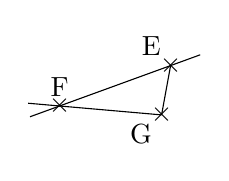
\begin{tikzpicture}[scale=1,every node/.style={scale=1}]

\draw (0,0) node [above]{F};
\draw (0,0) node {$\times$};
\draw (20:1.5) node [above left]{E};
\draw (20:1.5) node {$\times$};
\draw (-5:1.3) node [below left]{G};
\draw (-5:1.3) node {$\times$};

\draw (20:1.5)--(-5:1.3);
\draw (0,0)--+(175:0.4)--(-5:1.3);
\draw (0,0)--+(200:0.4)--(20:1.5)--+(20:0.4);

\draw (0,0.7); %pour donner un peu plus de hauteur à l'image
\end{tikzpicture} 
 			&  
    %manuel 6e, chapitre G3
\begin{tikzpicture}[scale=1,every node/.style={scale=1}]

\draw (0,0) node [above]{S};
\draw (0,0) node {$\times$};
\draw (50:1.5) node [above]{R};
\draw (50:1.5) node {$\times$};
\draw (5:2) node [below]{T};
\draw (5:2) node {$\times$};


\draw (0,1.9); %pour donner un peu plus de hauteur à l'image
\end{tikzpicture} 
			&
    %manuel 6e, chapitre G3
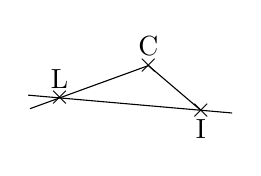
\begin{tikzpicture}[scale=1,every node/.style={scale=1}]

\draw (0,0) node [above]{L};
\draw (0,0) node {$\times$};
\draw (20:1.2) node [above]{C};
\draw (20:1.2) node {$\times$};
\draw (-5:1.8) node [below]{I};
\draw (-5:1.8) node {$\times$};

\draw (20:1.2)--(-5:1.8);
\draw (0,0)--+(175:0.4)--(-5:1.8)--+(-5:0.4);
\draw (0,0)--+(200:0.4)--(20:1.2);

\draw (0,0.7); %pour donner un peu plus de hauteur à l'image
\end{tikzpicture} 
			\\ \hline
    \end{tabular}\\[1em]

    
  %\newpage
  
   \item Compléter le tableau suivant :
   
   \vspace{1em}
   
   \renewcommand*\tabularxcolumn[1]{>{\centering\arraybackslash}m{#1}}
   \begin{ttableau}{\linewidth}{3}
    \hline
    \multicolumn{1}{|c|}{\textbf{Phrase}}	&	\multicolumn{1}{c}{\textbf{Phrase codée}}	&	\multicolumn{1}{|c|}{\textbf{Dessin}}			 	\\  \hline
    								&	Tracer $[UV]$							&	%manuel 6e, chapitre G3
\begin{tikzpicture}[scale=1,every node/.style={scale=1}]

\draw (0,0) node [above]{U};
\draw (0,0) node {$\times$};
\draw (2,0) node [above]{V};
\draw (2,0) node {$\times$};

\draw (0,0.7); %pour donner un peu plus de hauteur à l'image

\end{tikzpicture} 
		\\  \hline
    								&										&	%manuel 6e, chapitre G3
\begin{tikzpicture}[scale=1,every node/.style={scale=1}]

\draw (0,0) node [above]{A};
\draw (0,0) node {$\times$};
\draw (1.5,0) node [above]{M};
\draw (1.5,0) node {$\times$};
\draw (0,0)--(2.5,0);

\draw (0,0.7); %pour donner un peu plus de hauteur à l'image
\end{tikzpicture} 
		\\  \hline
   Tracer la droite passant par $S$ et $T$	&										&	%manuel 6e, chapitre G3
\begin{tikzpicture}[scale=1,every node/.style={scale=1}]

\draw (0,0) node [above]{S};
\draw (0,0) node {$\times$};
\draw (1.5,0) node [above]{T};
\draw (1.5,0) node {$\times$};

\draw (0,0.7); %pour donner un peu plus de hauteur à l'image
\end{tikzpicture} 
		\\  \hline
   								&										&	%manuel 6e, chapitre G3
\begin{tikzpicture}[scale=1,every node/.style={scale=1}]

\draw (0,0) node [above]{A};
\draw (0,0) node {$\times$};
\draw (1.5,0) node [above]{M};
\draw (1.5,0) node {$\times$};
\draw (-1,0)--(2.5,0);

\draw (0,0.7); %pour donner un peu plus de hauteur à l'image
\end{tikzpicture} 
	\\  \hline
   Tracer le segment d'extrémités $M$ et $N$	&									&	%manuel 6e, chapitre G3
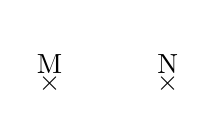
\begin{tikzpicture}[scale=1,every node/.style={scale=1}]

\draw (0,0) node [above]{M};
\draw (0,0) node {$\times$};
\draw (1.5,0) node [above]{N};
\draw (1.5,0) node {$\times$};

\draw (0,0.7); %pour donner un peu plus de hauteur à l'image
\end{tikzpicture} 
 	\\  \hline
   								&	Tracer $[KJ)$							&	%manuel 6e, chapitre G3
\begin{tikzpicture}[scale=1,every node/.style={scale=1}]

\draw (0,0) node [above]{K};
\draw (0,0) node {$\times$};
\draw (1.5,0) node [above]{J};
\draw (1.5,0) node {$\times$};

\draw (0,0.7); %pour donner un peu plus de hauteur à l'image
\end{tikzpicture} 
		\\  \hline
								&										&	%manuel 6e, chapitre G3
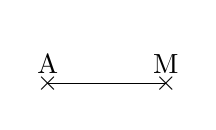
\begin{tikzpicture}[scale=1,every node/.style={scale=1}]

\draw (0,0) node [above]{A};
\draw (0,0) node {$\times$};
\draw (1.5,0) node [above]{M};
\draw (1.5,0) node {$\times$};
\draw (0,0)--(1.5,0);

\draw (0,0.7); %pour donner un peu plus de hauteur à l'image
\end{tikzpicture} 
	\\  \hline
   Tracer la demi-droite d'origine $U$ et 	&										&	%manuel 6e, chapitre G3
\begin{tikzpicture}[scale=1,every node/.style={scale=1}]

\draw (0,0) node [above]{O};
\draw (0,0) node {$\times$};
\draw (1.5,0) node [above]{U};
\draw (1.5,0) node {$\times$};

\draw (0,0.7); %pour donner un peu plus de hauteur à l'image
\end{tikzpicture} 
		\\
   passant par $O$					&										&										\\  \hline
   								&	Tracer $(BC)$							&	%manuel 6e, chapitre G3
\begin{tikzpicture}[scale=1,every node/.style={scale=1}]

\draw (0,0) node [above]{B};
\draw (0,0) node {$\times$};
\draw (1.5,0) node [above]{C};
\draw (1.5,0) node {$\times$};

\draw (0,0.7); %pour donner un peu plus de hauteur à l'image
\end{tikzpicture} 
		\\  \hline
  \end{ttableau}
  
   \end{enumerate} 

\end{activite}
%%%%%%%%%%%%%%%%%%%%%%%%%%%%%%%%%%%%%%%%%%%%%
